\documentclass[crop,tikz]{standalone}
\usetikzlibrary{backgrounds}
\colorlet{blue}{cyan}
\tikzset{
  inverted/.style = {
    color=white,
    background rectangle/.style={fill},
    show background rectangle
  }
}

\usepackage{amsmath}

\usetikzlibrary{patterns}
\colorlet{green}{green}

\begin{document}
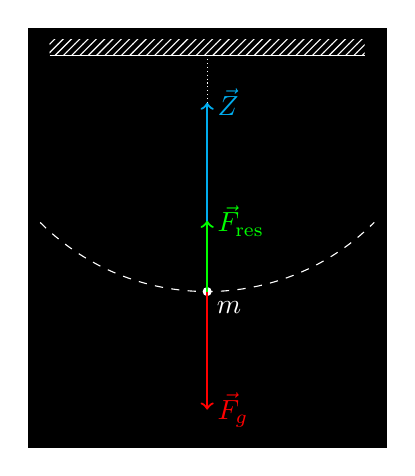
\begin{tikzpicture}[inverted,inverted]
  \pgfmathsetmacro{\Radius}{3};
  \pgfmathsetmacro{\Winkel}{1.5*30};
  \pgfmathsetmacro{\mass}{1};
  \pgfmathsetmacro{\gerde}{1.5};
  \pgfmathsetmacro{\phidot}{0.3};
  \pgfmathsetmacro{\mg}{\mass*\gerde};
  \pgfmathsetmacro{\FZp}{\mass*\Radius*\phidot};
  %
  \coordinate (O) at (0,0);
  \coordinate (N) at (0,{-\Radius});
  \coordinate (M) at (0,{-\Radius});
  %
  \pattern[pattern=north east lines,pattern color=white] (-2,0) rectangle (2,0.2);
  \draw (-2,0) -- (2,0);
  \draw[densely dotted] (O) -- (0,{-1.25*\Radius});
  \draw[dashed] ({270-\Winkel}:{\Radius}) arc ({270-\Winkel}:{270+\Winkel}:{\Radius});
  % mass
  \draw[fill] (M) circle (0.05) coordinate (mmax) node[below right] {$m$};
  % forces
  \draw[->,red,thick] (M) -- ++ (0,{-\mg}) node[right] {$\vec{F}_g$}; 
  \draw[->,blue,thick] (M) -- ++ (90:{\mg+\FZp}) node[right] {$\vec{Z}$};
  \draw[->,green,thick] (M) -- ++ (90:{\FZp}) node[right] {$\vec{F}_{\text{res}}$};
\end{tikzpicture}
\end{document}
